\documentclass[11pt]{article}           
\usepackage[UTF8]{ctex}
\usepackage[a4paper]{geometry}
\geometry{left=2.0cm,right=2.0cm,top=2.5cm,bottom=2.5cm}

\usepackage{xcolor}
\usepackage{paralist}
\usepackage{enumitem}
\setenumerate[1]{itemsep=0pt,partopsep=0pt,parsep=0pt,topsep=0pt}
\setitemize[1]{itemsep=0pt,partopsep=0pt,parsep=0pt,topsep=0pt}
\usepackage{comment}
\usepackage{booktabs}
\usepackage{graphicx}
\usepackage{float}
\usepackage{diagbox}
\usepackage{amsmath,amsfonts,graphicx,amssymb,bm,amsthm}
%\usepackage{algorithm,algorithmicx}
\usepackage[ruled]{algorithm2e}
\usepackage[noend]{algpseudocode}
\usepackage{fancyhdr}
\usepackage{tikz}
\usepackage{graphicx}
\usetikzlibrary{arrows,automata}
\usepackage[hidelinks]{hyperref}
\usepackage{extarrows}
\usepackage{lastpage}
\usepackage{totcount}
\setlength{\headheight}{14pt}
\setlength{\parindent}{0 in}
\setlength{\parskip}{0.5 em}
\usepackage{helvet}
\usepackage{dsfont}
\usepackage{threeparttable}
\usepackage{multirow}
\usepackage{tabularx}
% \usepackage{newtxmath}

\newtheorem{theorem}{Theorem}
\newtheorem{lemma}[theorem]{Lemma}
\newtheorem{proposition}[theorem]{Proposition}
\newtheorem{claim}[theorem]{Claim}
\newtheorem{corollary}[theorem]{Corollary}
\newtheorem{definition}[theorem]{Definition}
\newtheorem*{definition*}{Definition}

\newenvironment{problem}[2][Problem]{\begin{trivlist}
\item[\hskip \labelsep {\bfseries #1}\hskip \labelsep {\bfseries #2.}]\songti}{\hfill$\blacktriangleleft$\end{trivlist}}
\newenvironment{answer}[1][Solution]{\begin{trivlist}
\item[\hskip \labelsep {\bfseries #1.}\hskip \labelsep]}{\hfill$\lhd$\end{trivlist}}

\newcommand\1{\mathds{1}}
% \newcommand\1{\mathbf{1}}
\newcommand\R{\mathbb{R}}
\newcommand\E{\mathbb{E}}
\newcommand\N{\mathbb{N}}
\newcommand\NN{\mathcal{N}}
\newcommand\per{\mathrm{per}}
\newcommand\PP{\mathbb{P}}
\newcommand\dd{\mathrm{d}}
\newcommand\Var{\mathrm{Var}}
\newcommand\Cov{\mathrm{Cov}}
\newcommand{\Exp}{\mathrm{Exp}}
\newcommand{\arrp}{\xrightarrow{P}}
\newcommand{\arrd}{\xrightarrow{d}}
\newcommand{\arras}{\xrightarrow{a.s.}}
\newcommand{\arri}{\xrightarrow{n\rightarrow\infty}}

\title{Homework \#3}
\usetikzlibrary{positioning}

\begin{document}
\kaishu

\pagestyle{fancy}
\lhead{\CJKfamily{zhkai} 北京大学}
\chead{}
\rhead{\CJKfamily{zhkai} 2024年秋\ 社会统计学(张春泥)}
\fancyfoot[C]{\thepage\ /\ \pageref{LastPage} \\ \textcolor{lightgray}{最后编译时间: \today}}



\begin{center}
    {\LARGE \bf Homework 1}

    {姓名:方嘉聪\ \  学号: 2200017849}            % Write down your name and ID here.
\end{center}
\textcolor{gray}{\textbf{Note: }\underline{为了使自己日后复习方便我选择将题干一并打出, 望助教见谅.}}
\begin{problem}{1}
    职业性别隔离(occupational gender segregation)是指男性和女性集中从事不同的职业。通常体现为,男性集中从事的职业(即该职业男性比例高)的收入、地位较高;女性集中从事的职业(即该职业女性比例高)的收入、地位较低。以往研究发现,职业性别隔离是造成两性收入不平等的主要来源之一。作业1数据的表1是中国2010年全国人口普查分性别、非农职业小类的就业人口数。请你根据表1回答以下问题:
    \begin{enumerate}[label=(\arabic*)]
        \item 请对每个职业小类计算女性所占百分比(四舍五入取整数)和性别比{\kaishu(这一步的计算结果不必在作业纸上写出)}, 并报告女性集中从事的前五位职业和男性集中从事的前五位职业, 以及这些职业对应的女性百分比和性别比。{\kaishu(可采用文字叙述, 也可采用表格展示, 制表应注意规范性, 下同)}
        \item 将(1)计算得到的每类职业女性所占百分比(四舍五入取整数)按0-29\%、30-69\%、70-100\%将职业分为三组, 请问这属于什么分组?各组的真实组界、组距、组中心值分别是什么? 
        \item 根据(2)的分类, 如果将每类职业女性所占百分比为0-29\%的职业定义为“男性职业”、30-69\%定义为“中性职业”、70-100\%定义为“女性职业”。请你统计男性职业、中性职业、女性职业这三种职业性别类型分别在男性人口、女性人口、总人口中的分布, 并在同一张统计表中展示出来。
        \item 请依据(3)构造的统计表分别计算男性和女性人口的职业性别类型分布的众值和异众比率。
        \item 下图来自一篇有关中国职业性别隔离的论文, 其使用历次普查的职业小类数据计算了职业性别类型分布。请你根据(1)、(3)和(4), 从职业性别隔离的角度对中国男性和女性就业分布的特征进行简要总结, 并结合下图对总人口职业性别隔离的趋势进行简要描述{\kaishu(提示:言多必失, 写几句话意思表达清楚即可)}。
        \begin{figure}[H]
            \centering
            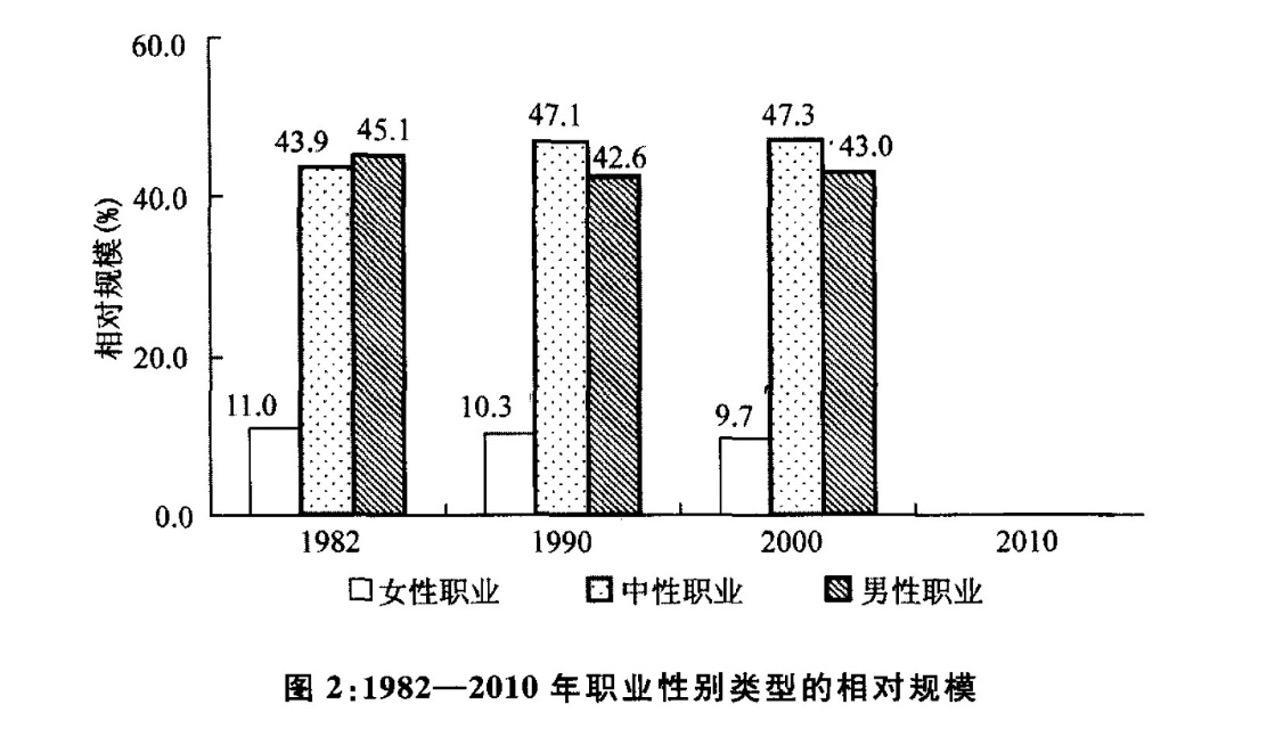
\includegraphics[width=0.6\textwidth]{./images/1.jpg}
        \end{figure}
    \end{enumerate}
\end{problem}
\begin{answer}
    \begin{enumerate}[label=(\arabic*)]
        \item 女性集中从事的前五位职业见表 \ref{tab:1.1}, 男性集中从事的前五位职业见表 \ref{tab:1.2}。注意其中性别比按 \underline{女性为100,男性对女性的比例} 计算。
        \begin{table}[H]
            \centering
            \caption{女性集中从事的前五位职业, 2010年普查}
            \label{tab:1.1}
            \begin{tabularx}{0.8\textwidth}{X>{\centering\arraybackslash}Xc}
                \hline
                \textbf{职业} & \textbf{女性百分比($\%$)} & \textbf{性别比 (男 : 女)} \\
                \hline
                幼儿教师 & 93 & 7.15 \\
                护理人员 & 93 & 7.45 \\
                保育、家庭服务人员 & 89 & 12.05\\
                抽纱、剌绣工艺品制作人员 & 97 & 14.76\\
                纺纱人员 & 76 & 30.74 \\
                \hline
            \end{tabularx}
        \end{table} 
        \begin{table}[H]
            \centering
            \caption{男性集中从事的前五位职业, 2010年普查}
            \label{tab:1.2}
            \begin{tabularx}{0.8\textwidth}{X>{\centering\arraybackslash}Xc}
                \hline
                \textbf{职业} & \textbf{女性百分比($\%$)} & \textbf{性别比 (男 : 女)} \\
                \hline
                船舶指挥和引航人员 & 6 & 1693.03 \\
                公(道)路运输机械设备操作及有关人员 & 6 & 1580.72 \\
                矿物开采人员 & 7 & 1244.46\\
                钻井人员 & 8 & 1205.69\\
                治安保卫人员 & 8 & 1100.79 \\
                \hline
            \end{tabularx}
        \end{table} 
        \item 属于不等距分组。各组的真实组界、组距、组中心值如下:
        \begin{itemize}
            \item 0-29\%:真实组界为$[-0.5\%, 29.5\%]$, 组距为$30\%$, 组中心值为$14.5\%$;
            \item  30-69\%:真实组界为$[29.5\%, 69.5\%]$, 组距为$40\%$, 组中心值为$49.5\%$;
            \item  70-100\%:真实组界为$[69.5\%, 100.5\%]$, 组距为$31\%$, 组中心值为$85.0\%$.
        \end{itemize}
        \item 统计表如表 \ref{tab:1.3}所示。
        \begin{table}[H]
            \centering
            \caption{男性人口、女性人口、总人口的职业性别类型分布, 2010年普查}
            \label{tab:1.3}
            \begin{tabularx}{\textwidth}{X>{\centering\arraybackslash}X>{\centering\arraybackslash}Xc}
                \hline
                \textbf{职业性别类型} & \textbf{男性人口中分布(\%)} & \textbf{女性人口中分布(\%)} & \textbf{总人口中分布(\%)} \\
                \hline
                男性职业 & 51.18 & 15.14 & 36.62 \\
                中性职业 & 44.82 & 66.96 & 53.76 \\
                女性职业 & 4.01 & 17.90 & 9.62 \\
                \multirow{2}{*}{合计} & 100.01 & 100.00 & 100.00 \\
                & (21898029人) & (14835332人) & (36733361人) \\
                \hline
            \end{tabularx}
        \end{table}  
        \item \begin{itemize}
            \item 男性人口的职业性别类型分布众值为男性职业, 异众比率为$48.83\%$
            \item 女性人口的职业性别类型分布众值为中性职业, 异众比率为$33.04\%$
        \end{itemize}
        \item \begin{itemize}
            \item 中国男性就业分布主要集中于男性职业与中性职业, 且男性职业与中性职业的占比相近, 其中最集中分布的是船舶、采矿、安保等相对重体力的职业。 而中国女性就业分布主要集中于中性职业(占比过半), 而相对不集中于女性职业, 其中最集中分布的是幼师、护理保育、纺织等职业。由此注意到存在一定的职业性别隔离现象。
            \item 从1982年-2010年, 男性职业和女性职业的比例逐渐减少, 中性职业的比例逐渐增加(查询原论文中2010年的数据发现2000-2010中性职业比例有相对更大的增加)。可见总人口职业性别隔离程度在逐渐减弱。
        \end{itemize}
    \end{enumerate}
\end{answer}

\begin{problem}{2}
    作业1数据中的表2是北京城市地区按月租房费用的家庭户户数的统计, 它来自中国2020年全国人口普查的汇总统计数据表。
    \begin{enumerate}[label=(\arabic*)]
        \item 请依据表2计算并报告北京城市地区租房家庭的月租房费用的均值、标准差、中位值和四分互差。{\kaishu(提示:缺下限组组中心值=该开口组真实上限-相邻组组距/2;缺上限组组中心值=该开口组真实下限+相邻组组距/2; 分组数据的方差和标准差计算可以利用组中值)}
        \item 试想若使用2020年全国人口普查的微观数据\footnote{即被调查者的原始个体数据}计算北京城市地区租房家庭的月租房费用均值和标准差, 数值与(1)完全一致吗?请说明你判断的理由。
    \end{enumerate}
\end{problem}
\begin{answer}
\begin{enumerate}[label=(\arabic*)]
    \item 根据所给数据, 并使用相关公式\[\text{Md} = L + \left( \frac{50\% - L\%}{U \% - L\%} \right) \times (U-L), ~~ \sigma^2 = \frac{\sum(x_{i} - \bar{x})^2}{N}, ~~ \bar{X} = \frac{\left( \sum n_{k} b_{k} \right)}{\sum n_{k}} = \sum p_{k} b_{k},~~ Q = Q_{3} - Q_{1}\]
    可得 \[\text{Md} = 2242.32,\quad \bar{X} = 3011.78, \quad \sigma = 2663.66, \quad Q = 4536.91 - 864.18 = 3672.73 \]
    注:在计算中将第一组的真实组限设置为$[-0.5,199.5)$, 第二组的真实组限设置为$[199.5,499.5)$, 最后一组缺上限, 计算得到的组中心值为 10999.5.
    \item 数值不会于(1)中完全一致。注意到(1)中的计算是基于分组数据的, 得到的的均值与方差是对原始数据的估计, 因此不会与(2)中使用微观数据(即原始个体数据)完全一致。
\end{enumerate}
\end{answer}

\begin{problem}{3}
    中国家庭追踪调查(CFPS)\footnote{关于中国家庭追踪调查:\href{http://www.isss.pku.edu.cn/cfps/}{http://www.isss.pku.edu.cn/cfps/}} 2016年调查对宗教信仰的测量如下:
    \begin{figure}[H]
        \centering
        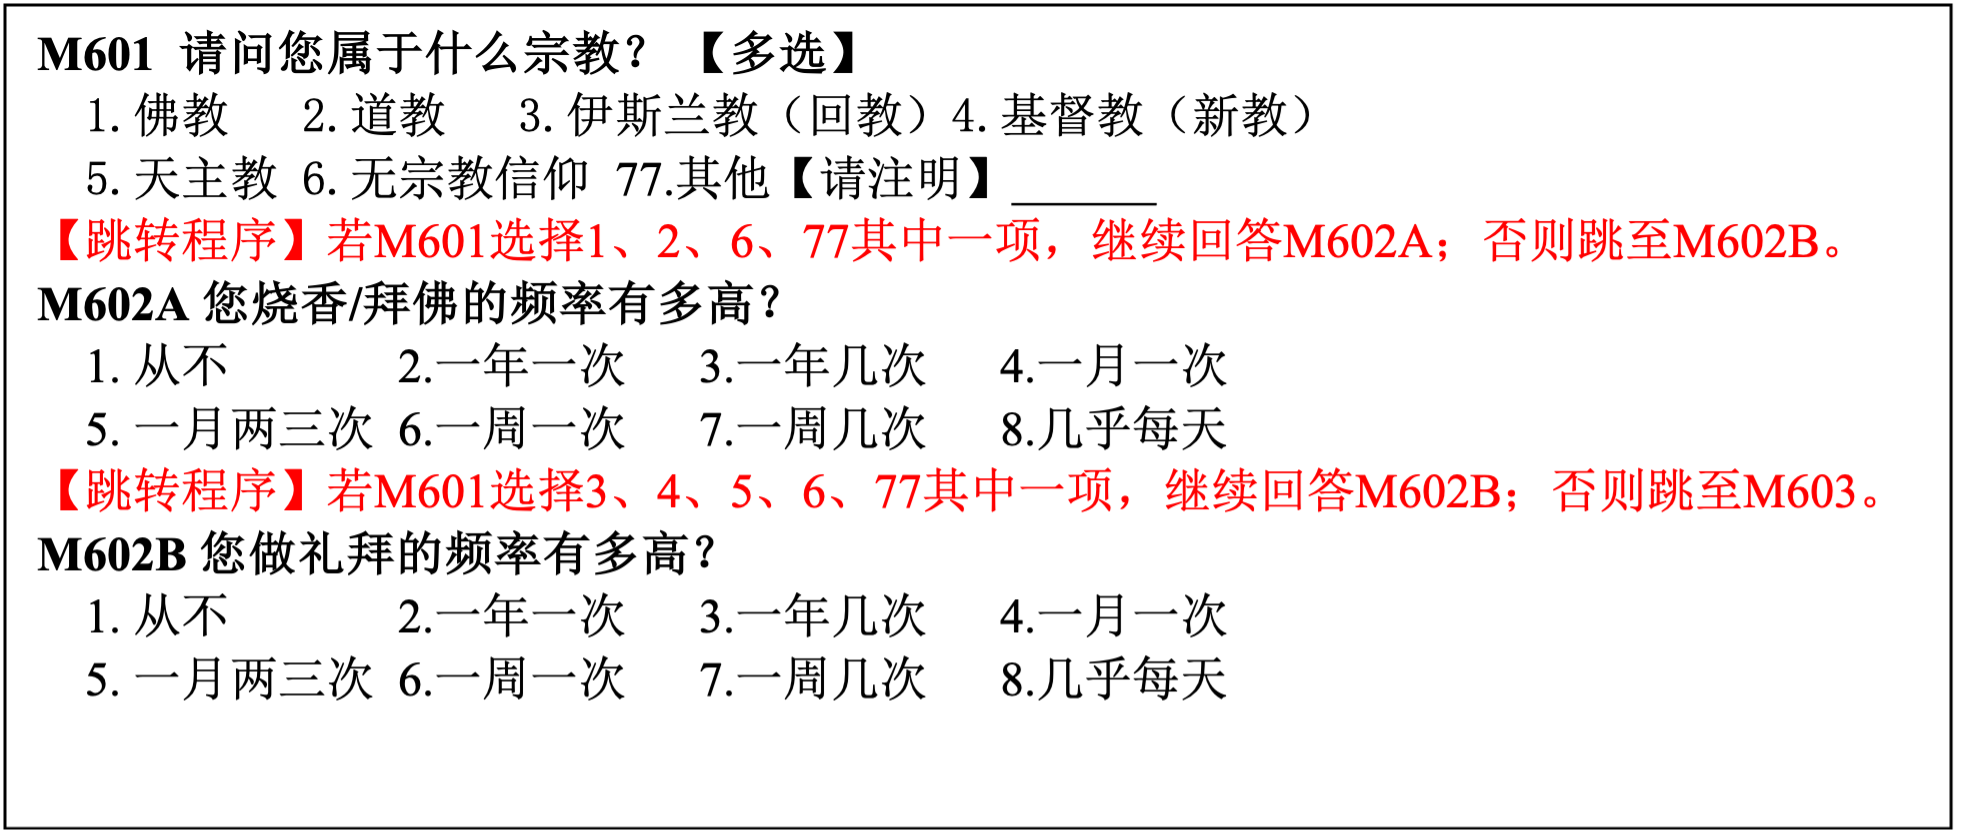
\includegraphics[width=0.6\textwidth]{./images/3.1.png}
    \end{figure}
    由于CFPS数据中只有极少数人回答信仰多种宗教信仰, 因此M601可以近似看作是单选题。表\ref{tab:3.1}统计了受访者回答M601宗教信仰题的频率分布:
    \begin{table}[H]
        \centering
        \caption{宗教信仰分布, CFPS 2016}
        \label{tab:3.1}
        \begin{tabularx}{0.8\textwidth}{Xc}
            \hline
            \textbf{宗教信仰} & \textbf{频率} \\
            \hline
            佛教 & 0.100 \\
            道教 & 0.005 \\
            伊斯兰教 & 0.011 \\
            基督教 & 0.020 \\
            天主教 & 0.004 \\
            其他 & 0.003 \\
            无宗教信仰 & 0.857 \\
            \multirow{2}{*}{合计} & 1.000 \\
            & (33193) \\
            \hline
        \end{tabularx}
        \begin{tablenotes}
            \footnotesize
            \item 注:由于信仰多种宗教的人极少, 已将这部分人排除, 此题可近似认为是单选题。
        \end{tablenotes}
    \end{table}
    根据表\ref{tab:3.1}受访者对宗教信仰的回答, 调查问卷进一步针对信仰佛教、道教、其他宗教和无宗教信仰者提问了他们烧香/拜佛(M602A)的频率;针对信仰伊斯兰教、基督教、天主教、其他宗教和无信仰者提问了他们做礼拜(M602B)的频率, 表\ref{tab:3.2}统计了各种信仰状况的人有过宗教实践(烧香/拜佛或者做礼拜的实践频率至少一年一次或以上)的频率
    \begin{table}[H]
        \centering
        \caption{各类信仰状况的人参与过宗教实践的频率, CFPS 2016}
        \label{tab:3.2}
        \begin{tabularx}{0.8\textwidth}{X>{\centering\arraybackslash}Xc}
            \hline
            \textbf{宗教信仰} & \textbf{烧香/拜佛} & \textbf{做礼拜} \\
            \hline
            佛教 & 0.87 & / \\
            道教 & 0.81 & / \\
            伊斯兰教 & / & 0.78\\
            基督教 & / & 0.82\\
            天主教 & / & 0.62\\
            其他 & 0.68  & 0.09 \\
            无宗教信仰 & 0.31 & 0.01\\
            \hline
        \end{tabularx}
        \begin{tablenotes}
            \footnotesize
            \item 注:“参与过宗教实践”定义为烧香/拜佛或者做礼拜的频率在一年一次及以上, 具体包括:一年一次、一年几次、一月一次、一月两三次、一周一次、一周几次、几乎每天。已排除掉信仰多种宗教的人。“/”表示不适用(已跳答)。
        \end{tablenotes}
    \end{table} 
    若表\ref{tab:3.1}和表\ref{tab:3.2}统计的频率可以作为概率的近似值, 问:
    \begin{enumerate}[label=(\arabic*)]
        \item 从CFPS调查样本中任抽取一人, 他/她有烧香/拜佛行为的概率是多少?
        \item 已知一名受访者烧香/拜佛的情况下, 他/她是无宗教信仰者的概率是多少?
        \item 已知一名受访者做礼拜的情况下, 他/她是基督徒的概率是多少?
    \end{enumerate}
\end{problem}
\begin{answer}
    \begin{enumerate}[label=(\arabic*)]
        \item 记事件$A_1 = \{\text{他/她有烧香/拜佛行为}\}$, 则有\[\PP(A_1) = 0.100 \times 0.87 + 0.005 \times 0.81 + 0.003 \times 0.68 + 0.857 \times 0.31 \approx 0.36\]
        \item 记事件$A_2 = \{\text{他/她有烧香/拜佛行为}\}, B_2 = \{\text{他/她是无宗教信仰者}\}$, 那么\begin{align*}
            \PP(B_2|A_2) = \frac{\PP(A_2 B_2)}{\PP(A_2)} = \frac{0.31 \times 0.857}{0.36} \approx 0.74
        \end{align*}
        故已知一名受访者烧香/拜佛的情况下,他/她是无宗教信仰者的概率是0.74.
        \item 记事件$A_3 = \{\text{他/她做礼拜}\}, B_3 = \{\text{他/她是基督徒}\}$, 那么\begin{align*}
            \PP(A_3) =  0.011 \times 0.78 + 0.020 \times 0.82 &+ 0.004 \times 0.62 + 0.003 \times 0.09 + 0.857 \times 0.01 = 0.0363 \\
            \PP(B_3|A_3) &= \frac{\PP(A_3 B_3)}{\PP(A_3)} = \frac{0.82 \times 0.020}{0.0363} \approx 0.45
        \end{align*}
        故已知一名受访者做礼拜的情况下,他/她是基督徒的概率是0.45.
    \end{enumerate}
\end{answer}
\end{document}